\chapter{Golden Ratio}

In mathematics and the arts, two quantities are in the golden ratio if their ratio is the same as the ratio of their sum to the larger of the two quantities, i.e.~their maximum. The figure on the right illustrates the geometric relationship. Expressed algebraically, for quantities $a$ and $b$ with $a > b$,
\begin{equation}
 \frac{a+b}{a} = \frac{a}{b} \ \stackrel{\text{def}}{=}\ \varphi,
\end{equation}
where the Greek letter $\varphi$ represents the golden ratio. Its value is:
\begin{equation}
\varphi = \frac{1+\sqrt{5}}{2} = 1.61803\,39887\ldots.
\end{equation}

\section{History}

Ancient Greek mathematicians first studied what we now call the golden ratio because of its frequent appearance in geometry. The division of a line into ``extreme and mean ratio'' (the golden section) is important in the geometry of regular pentagrams and pentagons. Euclid's Elements  provides the first known written definition of what is now called the golden ratio: ``A straight line is said to have been cut in extreme and mean ratio when, as the whole line is to the greater segment, so is the greater to the less.'' Euclid explains a construction for cutting (sectioning) a line ``in extreme and mean ratio'', i.e., the golden ratio. (See Figure~\ref{fig:line:golden}.) Throughout the Elements, several propositions (theorems in modern terminology) and their proofs employ the golden ratio.

\begin{figure}[hbt!]\centering
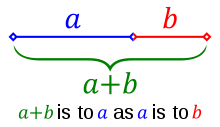
\includegraphics[width=.3\textwidth]{220px-Golden-ratio-line}
\caption{Line segments in the golden ratio}
\label{fig:line:golden}
\end{figure}

\begin{figure}[hbt!]\centering
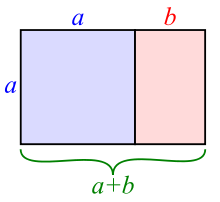
\includegraphics[width=.3\textwidth]{SimilarGoldenRectangles}
\caption{Golden rectangles}
\end{figure}



\section{Calculation}
Two quantities $a$ and $b$ are said to be in the golden ratio $\varphi$ if:
\begin{equation}
 \frac{a+b}{a} = \frac{a}{b} = \varphi.
\end{equation}

One method for finding the value of $\varphi$ is to start with the left fraction. Through simplifying the fraction and substituting in $\frac{b}{a} = \frac{1}{\varphi}$,
\begin{equation}
\frac{a+b}{a} = 1 + \frac{b}{a} = 1 + \frac{1}{\varphi},
\end{equation}

By definition, it is shown that
\begin{equation}
 1 + \frac{1}{\varphi} = \varphi. 
\end{equation}
Multiplying by $\varphi$ gives
\begin{equation*}
\varphi + 1 = \varphi^2
\end{equation*}
which can be rearranged to
\begin{equation*}
{\varphi}^2 - \varphi - 1 = 0.
\end{equation*}
Using the quadratic formula, two solutions are obtained:
\begin{equation*}
\varphi = \frac{1 + \sqrt{5}}{2} = 1.61803\,39887\dots
\end{equation*}
and
\begin{equation*}
\varphi = \frac{1 - \sqrt{5}}{2} = -0.6180\,339887\dots
\end{equation*}
Because $\varphi$ is the ratio between positive quantities $\varphi$ is necessarily positive:
\begin{equation*}
\varphi = \frac{1 + \sqrt{5}}{2} = 1.61803\,39887\dots .
\end{equation*}

Different representations of the golden ratio are given in Table~\ref{tab:goldenratio}.

\begin{table}[hbt!]\centering
\caption{Number representations of the golden ratio}
\label{tab:goldenratio}

\begin{tabular}{|l|l|}
\hline
Form & Representation\\\hline
Binary & 1.1001111000110111011\ldots\\\hline
Decimal & 1.6180339887498948482\ldots\\\hline
Hexadecimal	& 1.9E3779B97F4A7C15F39\ldots\\\hline
Continued fraction & $1 + \cfrac{1}{1 + \cfrac{1}{1 + \cfrac{1}{1 + \cfrac{1}{1 + \ddots}}}}$\\[6ex]\hline
Algebraic form & $\displaystyle\frac{1 + \sqrt{5}}{2}$\\[2ex]\hline
Infinite series & $\displaystyle\frac{13}{8}+\sum_{n=0}^{\infty}\frac{(-1)^{(n+1)}(2n+1)!}{(n+2)!\,n!\,4^{(2n+3)}}$\\[2ex]\hline
\end{tabular}
\end{table}
